
\section{Задача торга двух игроков.}

% использовать букву f для выигрыша - исправить в лекции 2 для полноты картины.



\subsection{Определение задачи торга.}

Попробуем разобрать простейший случай, когда полезности не передаются.
У нас будет всего \indef{два} игрока. Либо каждый из них работает
в одиночку, либо формируется большая коалиция. Большая, в данном случае,
- это из обоих игроков.

Соответственно, описание задачи торга состоит из двух объектов:

\begin{mydef} Точка разногласия \index{Точка разногласия} (disagreement point) - это вектор
платежей, получаемых игроками, если кооперации не будет. \end{mydef}

\begin{mydef} Множество доступных платежей \index{Множество доступных платежей} - это множество возможных платежей,
которые могут получить игроки если скооперируются. \end{mydef}

\begin{figure}[htbp]
	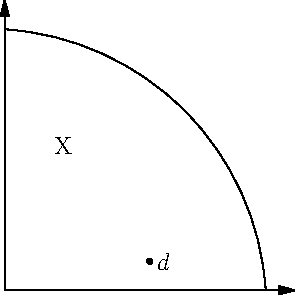
\includegraphics{coop_feasible.pdf}
\end{figure}


С формальной математической точки зрения задача торга задается парой
$(X,d)$, где $X$ - множество доступных платежей, а $d$ - точка разногласия.

Это несколько больше, чем коалиционная игра двух игроков в характеристической
форме. Игра в характеристической форме предполагает, что множество
$X$ имеет вид $X=\{(x_{1},x_{2})|x_{1}+x_{2}\leq v(N)\}$. В задаче
торга множество $X$ в принципе может иметь любую форму. Поэтому можно
считать, что это не деньги, а полезность. В этих лекциях полезность
измеряется в улыбках.

Впрочем, чаще всего предполагают, что множество доступных платежей не совсем
произвольно, а удовлетворяет требованиям:
\begin{itemize}
\item Замкнуто;
\item Выпукло;
\item Ограничено сверху, т.е. существует такая точка $a=(a_{1},a_{2})$
на плоскости, что все множество $X$ лежит юго-западнее точки $a$;
\item Содержит точку $d$.
\end{itemize}
Мы будем считать, что эти требования выполнены.

Что означает решить задачу торга? Для данной конкретной задачи это
означает выбрать наилучшую точку $x^{*}$из $X$. Но нас интересует
не решение конкретной задачи торга, а некое правило которое позволяет
решать любую задачу торга. Наше правило каждой задаче торга $(X,d)$
сопоставляет некий <<наилучший>> дележ $x^{*}$. С математической
точки зрения, правило дележа - это функция $f$. Соответственно, область
определения функции $f$ - это всевозможные задачи торга, т.е. всевозможные
пары $(X,d)$. 

Пусть $x^{*}$ - это предлагаемый игрокам дележ, т.е. $x^{*}=f((X,d))$.

Чего бы мы хотели от хорошего правила дележа $f$?
\begin{itemize}
\item 
\phantomsection \label{irationality}
Индивидуальная рациональность. \index{Индивидуальная рациональность} Каждый игрок должен получать не меньше,
чем в точке разногласия, $x^{*}\geq d$, т.е. $x_{1}^{*}\geq d_{1}$,
$x_{2}^{*}\geq d_{2}$.
\item Эффективность.\index{Эффективность} Дележ $x^{*}$ должен быть Парето-оптимален. Другими
словами, не существует такой точки $x^{'}$, которая была была бы
для обоих игроков не хуже, а кому-то даже лучше. Формально, не существует
такая точка $x^{'}\neq x^{*}$, что $x^{'}\geq x^{*}$.
\item Симметрия. \index{Симметрия} Если игроки одинаковые (т.е. множество $X$ симметрично
относительно прямой $x_{1}=x_{2}$, и в случае разногласия игроки
получают одинаковый выигрыш $d_{1}=d_{2}$), то $x_{1}^{*}=x_{2}^{*}$.
\item 
\phantomsection \label{scale_invariance}
Нечувствительность к смене масштаба. \index{Нечувствительность к смене масштаба} Пусть есть две задачи торга $(X,d)$
и $(X^{'},d^{'})$, которые отличаются масштабом. Скажем в первой
полезность измерялась в улыбках, а во второй - в улыбочках (одна улыбочка
это $10^{-3}$ улыбок). В этом случае хотелось бы, чтобы решения этих
задач также отличались только сменой масштаба. И более формально:
пусть $X'=aX+b$ и $d'=ad+b$, где $a$ и $b$ - произвольные константы.
Мы говорим, что решение $f$ нечувствительно к смене масштаба, если
$f(X')=af(X)+b$.%
\footnote{Это требование называется у В.И. Данилова скалярной ковариантностью.
Страшно, да?%
}
\item 
\phantomsection \label{3_invariance}
Независимость от третьих альтернатив. \index{Независимость от третьих альтернатив} Если при доступных точках $x$,
$y$, $z$ правило выбирало $x$, то при доступных $x$ и $y$ правило
тоже должно выбирать $x$.
\end{itemize}
Существуют ли решение которое всегда удовлетворяет всем этим требованиям?
Правильный ответ в студию!


\subsection{Решение Нэша}

Для начала введем понятие:

\begin{mydef}
Вектор $y$ называется бонусом от кооперации \index{Бонус от кооперации} при дележе $x$, если $y=x-d$.  Это выигрыш игроков от кооперации по сравнению с точкой разногласия,
\end{mydef}

Нэш предложил странное на первый взгляд решение: 

\begin{mydef} \indef{Решение Нэша} \index{Решение Нэша} - это точка $x_{Nash}$, которая
лежит в $X$ и максимизирует произведение бонусов от кооперации. Т.е.
$(x_{1},x_{2})_{Nash}$ максимизирует функцию $f(x_{1},x_{2})=(x_{1}-d_{1})(x_{2}-d_{2})$.
\end{mydef}

\begin{figure}[htbp]
	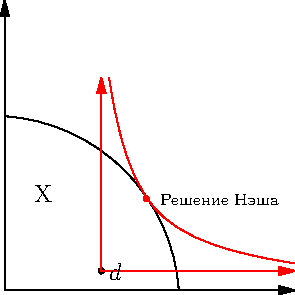
\includegraphics{coop_nash.pdf}
\end{figure}



Давайте попробуем найти решение Нэша в задаче про носки. Напомним
текст:
\begin{myex} Левые и правые носки ничем не отличаются. Пара носков стоит 60 рублей. Один носок ничего не стоит. У Андрея - три носка, у Бориса - пять носков. Здесь $N=\{$Андрей,Борис$\}$, $v($Андрей$)=60$, $v($Борис$)=120$, $v($Андрей, Борис$)=240$.
\end{myex}

В нашем случае, точка несогласия, $d=(60,120)$, а переговорное множество
$X=\{(x_{1},x_{2})|x_{1}+x_{2}\leq240\}$.

Обозначим бонус от кооперации буквой $y_{i}$, т.е. $y_{i}=x_{i}-d_{i}$.
Решение Нэша максимизирует величину $y_{1}\cdot y_{2}$ при ограничении
$y_{1}+y_{2}\leq60$. В силу симметрии $y_{1}=y_{2}=30$.

Значит Нэша предлагает поделить совокупных доход как $(90,150)$.
Что, кстати говоря, совпадает с вектором Шепли и интуитивным дележом
$3:5$.

Оказывается, что:

\begin{myth} Решение Нэша - это единственное решение, удовлетворяющиее
требованиям \hyperref[irationality]{индивидуальной рациональности}, \hyperref[Pareto]{эффективности}, \hyperref[symmetry]{симметричности}, \hyperref[scale_invariance]{нечувствительности к смене масштаба} и \hyperref[3_invariance]{независимости от третьих альтернатив}.
\end{myth}



\begin{proof} 

Для начала рассмотрим задачу торга, где $d=(0;0)$, а переговорное
множество $Y={(x_{1},x_{2})|x_{1}+x_{2}\leq2}$. Игроки симметричны,
значит должны получить одинаковый выигрыш. Единственное симметричное
Парето-оптимальное решение - это $(1,1)$. Решение Нэша именно это и предлагает. 

\begin{figure}[htbp]
	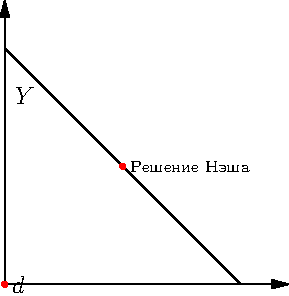
\includegraphics{coop_neproof1.pdf}
\end{figure}



Теперь рассмотрим произвольную задачу торга, $(X,d)$. Идея состоит в том, чтобы так подгадать смену масштаба, чтобы $X'$, отмасштабированное множество доступных альтернатив, оказалось внутри упомянутого множества $Y$ и точка $(1,1)$ была бы у них общей. В силу независимости от третьих альтернатив мы обязаны в отмасштабированном $X'$ выбрать точку $(1,1)$ (она была наилучшей в более крупном множестве $Y$). Значит в исходном множестве $X$ мы обязаны выбирать ту точку, которая после смены масштаба стала точкой $(1,1)$.

\begin{figure}[htbp]
	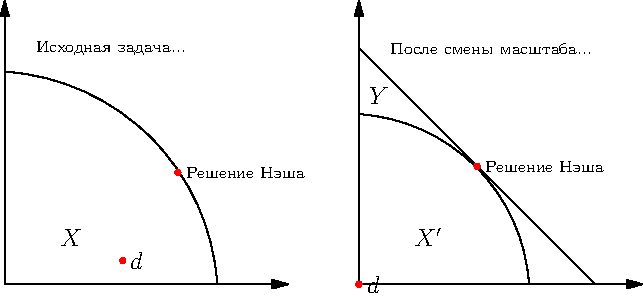
\includegraphics{coop_neproof2.pdf}
\end{figure}


Какая смена масштаба нам нужна? Нужно, чтобы при смене масштаба $d\to (0;0)$ и $x_{NE}\to (1,1)$. Тогда как раз окажется, что правило выбирающее $(1,1)$ в новом $X'$ будет выбирать решение Нэша в исходном $X$. Такая смена масштаба существует. Можно даже предъявить явную формулу (хотя она и не очень нужна, но пусть будет): $x_{i}^{'}=(x_{i}-d_{i})/(x_{NE,i}-d_{i})$. При этом чудесным образом автоматически получается, что новое $X'$ лежит внутри $Y$. 


Почему же окажется, что $X'$ лежит внутри $Y$? На множестве $X$ дележ $x_{NE}$ было равновесием по Нэшу, значит $X$ касалось гиперболы $(x_{1}-d_{1})\cdot (x_{2}-d_{2})=c$. Следовательно, $X$ лежало левее и ниже касательной к этой гиперболе. При смене масштаба касательная аккурат совпадет с прямой $x_{1}^{'}+x_{2}^{'}=2$. В этом можно убедиться выписав ее старое уравнение и сменив масштаб.

\end{proof}


\subsection{Решение Калаи-Смородинского}

Условие независимости от третьих альтернатив может быть рациональным,
но оно зачастую нарушается в реальности. Давайте рассмотрим такой
пример.

Вовочка и Петечка долго спорили о том, кто является самой красивой
девушкой в их классе, Маша или Аня. После долгого спора они пришли
к общему мнению, что самая красивая - Маша. После этого спора Вовочка
и Петечка неожиданно вспомнили про Памеллу Андерсон. А вспомнив про
Памеллу Андерсон, решили, что все-таки, самая красивая - Аня.

На этот пример можно, конечно, возразить, что Памелла Андерсон не
училась в классе Вовочки и Петечки. И это, следовательно, не совсем
независимость от третьих альтернатив. Но идея остается. Чтобы сделать
выбор между несколькими объектами нужно свести многомерные характеристики
объектов к одной единственной лучше-хуже. И вот-это правило сведения
оказывается очень неустойчиво. На него влияет реклама или просто упоминание
третьей альтернативы.

Еще пример. Вы выбирали мобильный телефон и сомневались между А и
Б. И склонились к выбору А. Потом в журнале прочли про то, что есть
такая крутая модель С. Крута она своим дизайном. Вам дизайн С понравился.
И вы сменили свой выбор в пользу Б, потому, что дизайн Б больше похож
на крутой дизайн С. Сама модель С для вас была хуже, чем А и Б, так
как у нее существенно выше цена. Но критерий сведения многомерной
характеристики телефона к одномерному хуже-лучше поменялся просто
из-за самого наличия С.

Решение Калаи-Смородинского заменяет требование независимости от третьих
альтернатив на индивидуальную монотонность. Чтобы проще описать
индивидуальную монотонность определим пару функций:
\begin{itemize}
\item $m_{1}(X,d)$ - это наибольший возможный для первого игрока бонус
от кооперации, при котором бонус второго игрока неотрицателен. И,
аналогично, 
\item $m_{2}(X,d)$ - это наибольший возможный для второго игрока бонус
от кооперации, при котором бонус первого игрока неотрицателей.
\end{itemize}


\phantomsection \label{imonotonicity}
Индивидуальная монотонность (для первого игрока).\index{Индивидуальная монотонность} Допустим у нас есть
две задачи торга, $(X,d)$ и $(X^{'},d^{'})$. Если множество дележей $X^{'}$ больше, чем $X$, но максимальный бонус от кооперации для второго игрока одинаковый, то с точки зрения первого игрока задача $(X^{'},d^{'})$ должна быть лучше задачи $(X,d)$. Формально, если $X\subset X^{'}$ и $m_{2}(X,d)=m_{2}(X^{'},d^{'})$, то $x^{*'}_{1}\geq x^{*}_{1}$.


\begin{mydef}Решение Калаи-Смородинского, $x_{KS}$ - это 
Парето-оптимальное решение, которое делит бонусы от кооперации в пропорции
$m_{1}(X,d):m_{2}(X,d)$.\end{mydef}

\begin{figure}[htbp]
	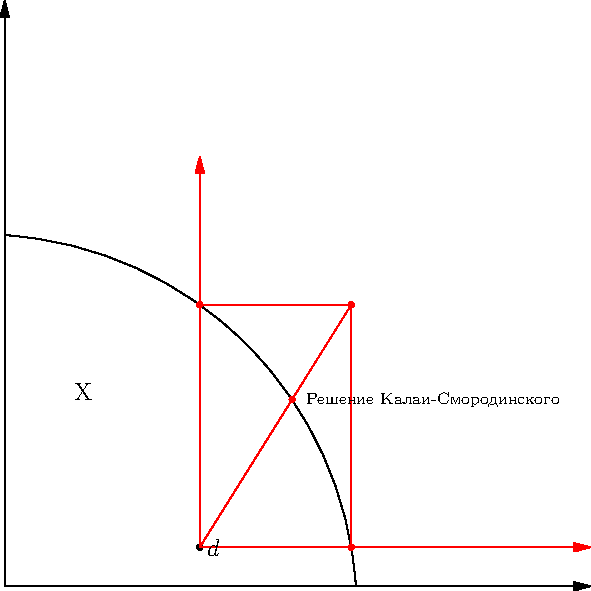
\includegraphics{coop_ks.pdf}
\end{figure}


Как можно было догадаться, верна следующая характеристика решения Калаи-Смородинского:
\begin{myth} Решение Калаи-Смородинского - это единственное решение, удовлетворяющиее
требованиям \hyperref[irationality]{индивидуальной рациональности}, \hyperref[Pareto]{эффективности}, \hyperref[symmetry]{симметричности}, \hyperref[scale_invariance]{нечувствительности к смене масштаба} и \hyperref[imonotonicity]{индивидуальной монотонности}.
\end{myth}

Найдем решение Калаи-Смородинского в задаче про Носки. Точка несогласия,
$(60,120)$. Общий бонус от кооперации - $60$. Поскольку деньги можно
передавать, то максимальный бонус каждого игрока от кооперации также
равен $60$, т.е. $m_{1}=m_{2}=60$. Делим общий бонус от кооперации
в пропорции $60:60$, т.е. поровну. Каждый получает бонус по $30$.
Итоговый дележ $(90,150).$ Что совпадает с решением Нэша, а заодно
и с вектором Шепли.


\subsection{Связь с некооперативной теорией игр.}

Неплохо бы навести какой-то мостик между кооперативной и некооперативной
теориями. Иначе они кажутся совершенно оторванными, хотя решают похожие
задачи.

Представим себе, что торг проходит так:

Период 1. Игрок А предлагает игроку Б любой дележ из $X$. Если Б
согласен, то игра заканчивается. Если игрок Б не согласен, то начинается
период 2.

Период 2. Игрок Б предлагает играку А любой дележ из $X$. Если А
согласен, то игра заканчивается. Если игрок А не согласен, то начинается
период 3.

... и так далее.

Дополнительно добавим в игру ураган. После окончания каждого периода (перед началом следующего) с вероятностью $p\in (0;1)$ начинается ураган. \index{Ураган} В случае урагана игра
принудительно заканчивается и если игроки не успели договориться,
то они получают выигрыш из точки несогласия $d$. Уточним, что дисконтирования
нет.

Зачем нам нужен ураган? Чтобы стимулировать игроков прийти к соглашению
побыстрее. В каком-то смысле он заменяет дисконтирование. Рубль сейчас
лучше чем обещание рубля завтра, т.к. до завтра может начаться ураган
и обещание не будет исполнено.

Найдем равновесие по Нэшу совершенное в подыграх (SPNE) \index{Равновесие по Нэшу совершенное в подыграх} для каждого
$p$. Обозначим вектор платежей, которые получают игроки, как $x_{SPNE}(p)$.

Оказывается, что:

\begin{myth} Решение Нэша в задаче торга является пределом равновесий
по Нэшу совершенных в подыграх, $x_{Nash}=\lim_{p\to 0}x_{SPNE}(p)$.
\end{myth}

\begin{proof}

Как мы уже делали, будем рассматривать бонусы от кооперации. Т.е.,
например, если начался ураган, то игроки получают $(0;0)$. 

Найдем SPNE для произвольного $p$. Если игра дошла до 3-го периода,
то она ничем не отличается от изначальной игры. Поэтому сначала найдем
совсем простое равновесие, в котором предлагаемый каждым игроком дележ
все время один и тот же. Наше равновесие имеет такой вид: При своем
ходе первый игрок всегда будет предлагать один и тот же вектор бонусов
$x^{*}=(x_{1}^{*},x_{2}^{*})$, а второй игрок при своем ходе будет
предлагать вектор бонусов $y^{*}=(y_{1}^{*},y_{2}^{*})$. При этом
$x_{2}^{*}$ - это наименьший бонус, одобряемый вторым игроком, а
$y_{1}^{*}$ - наименьший бонус одобряемый первым игроком. 

Равновесная траектория выглядит так: первый игрок предлагает $x^{*}=(x_{1}^{*},x_{2}^{*})$. Второй игрок соглашается. Игра оканчивается без наступления урагана.

Для поиска SPNE указанного вида применим принцип одноразового отклонения: \index{Принцип одноразового отклонения}

\begin{myth}
Профиль стратегий является равновесием по Нэшу совершенным в подыграх
если и только если ни одному игроку ни в одной подыгре не выгодны
одноразовые отклонения. Под одноразовым отклонением от стратегии $s$
подразумевается любая стратегия $s'$, которая отличается от стратегии
$s$ лишь в один момент времени.\footnote{Для тех, кто плохо помнит, что это значит, приведем пример.
Пусть имеется стратегия $s=\{$в первой партии сделать ход $a$, в последующих
партиях сделать ход, сделанный в первой партии$\}$. Тогда стратегия
$s'=\{$в первой партии сделать ход $b$, в последующих партиях сделать
ход, сделанный в первой партии$\}$ является одноразовым отклонением
от стратегии $s$. Напомним также, что проверять нужно не только равновесную
траекторию, но и любую другую.%
}.

\end{myth}


Проверяем возможность неодобрения высокого платежа. Итак, пусть первый
игрок предложил дележ $x=(x_{1},x_{2}^{*}+\Delta)$, не обязательно
равновесный! Если второй соглашается (согласно своей стратегии), то
он получает бонус $x_{2}^{*}+\Delta$. Если второй игрок делает одноразовое
отклонение (и, стало быть, не соглашается), то: С вероятностью $p$
игроки получают бонус ноль. С вероятностью $(1-p)$ начинается
следующий период, в котором второй игрок (вернувшись к своей стратегии)
предлагает вектор $y=(y_{1}^{*},y_{2}^{*})$ и первый игрок соглашается. 

Чтобы одноразовое отклонение не было выгодно: $x_{2}^{*}+\Delta\geq(1-p)y_{2}^{*}$
для всех $\Delta\geq0$. 

Проверяем возможность одобрения низкого платежа. Итак, пусть первый
игрок предложил дележ $x=(x_{1},x_{2}^{*}-\Delta)$, не обязательно
равновесный! Если второй не соглашается (согласно своей стратегии),
то он получает ожидаемый бонус $(1-p)y_{2}^{*}$. Если второй
игрок делает одноразовое отклонение (и, стало быть, соглашается),
то он получает $x_{2}^{*}-\Delta$.

Чтобы одноразовое отклонение не было выгодно: $(1-p)y_{2}^{*}\geq x_{2}^{*}-\Delta$
для всех $\Delta<0$

Получаем уравнение 

\begin{equation}
\label{eq:spne1}
x_{2}^{*}=(1-p)y_{2}^{*}
\end{equation}

Аналогично для другого игрока, 
\begin{equation}
\label{eq:spne2}
y_{1}^{*}=(1-p)x_{1}^{*}
\end{equation}



Пока что мы получили два уравнения на 4 неизвестных. Еще два получить
совсем просто: бонусы $x^{*}$ и $y^{*}$ в нашем профиле стратегий
должны быть парето-оптимальными, т.к. в противном случае первый игрок
сменит его на $(x_{1}^{*}+\Delta,x_{2}^{*})$, а второй игрок немедленно
одобрит такой дележ.

Честно говоря, надо доказывать, что других существенно отличающихся
равновесий нет, но сейчас мы этого делать не будем.

Итак, при любой вероятности $p$ равновесный (в смысле SPNE)
платеж можно найти из условий:

$x^{*}$ и $y^{*}$ Парето-оптимальны, $x_{2}^{*}=(1-p)y_{2}^{*}$,
$y_{1}^{*}=(1-p)x_{1}^{*}$ 

Это 4 уравнения на 4 неизвестных (Парето-оптимальность означает, что
точки лежат на границе переговорного множества). 

Заметим, что $x_{1}^{*}x_{2}^{*}=y_{1}^{*}y_{2}^{*}$ при любом $p$,
т.е. произведения бонусов, получаемых игроками равны. Графически это
означает, что предложения $x^{*}$ и $y^{*}$ находятся на пересечении
границы переговорного множества и гиперболы $b_{1}b_{2}=const$.
Значение константы $const$ определяется
значением вероятности $p$.


\begin{figure}[htbp]
   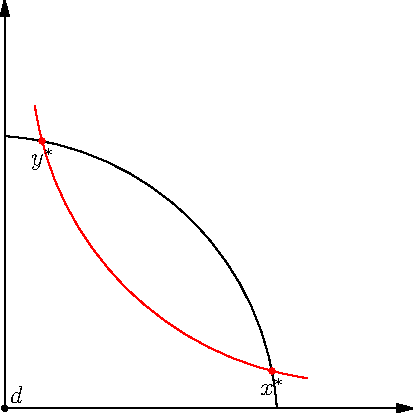
\includegraphics{coop_noncop0.pdf}
\end{figure}


Теперь возьмем произвольную последовательность $p_{n}\downarrow 0$ и посмотрим, что происходит с предложениями $x^{*}(p_{n})$ и $y^{*}(p_{n})$. Из уравнений \ref{eq:spne1} и \ref{eq:spne2} ясно, что точки $x^{*}(p_{n})$ и $y^{*}(p_{n})$ сближаются. Это означает, что гипербола, на которой они лежат сдвигается вправо-вверх. В пределе должны получать единственное решение, и оно совпадает с решением Нэша.

\begin{figure}[htbp]
   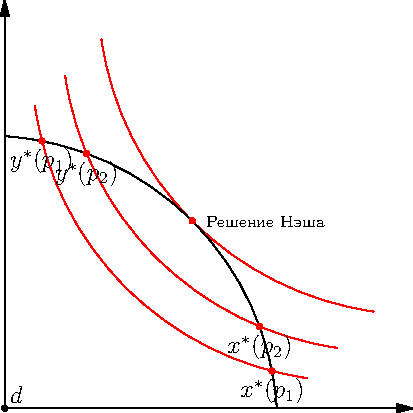
\includegraphics{coop_noncop.pdf}
\end{figure}


\end{proof}

